\documentclass[a4paper,11pt,titlepage,abstract,numbers=noenddot,automark,mnsy,intlimits,rgb,dvipsnames]{report}
\usepackage[hidelinks, colorlinks=true, urlcolor=blue, linkcolor=black, citecolor=blue]{hyperref}
\usepackage[english]{babel}
\usepackage{unicode-math}
\usepackage{xunicode}
\usepackage{url}
\usepackage{cite}
\usepackage{graphicx}
\usepackage[justification=centering, labelfont=bf]{caption}
\usepackage{float}
\usepackage{pgfgantt}
\usepackage{marvosym}
\usepackage{siunitx}
\usepackage{multirow}
\usepackage[nottoc]{tocbibind}
\usepackage{indentfirst}
\usepackage{afterpage}
\usepackage{minted}
\usepackage{tabularx}
\usepackage{tikz}
\usepackage[toc,page]{appendix}
\usepackage{svg}
\usetikzlibrary{arrows,positioning}
\usepackage{fontspec}
\usepackage{parskip}
\usepackage{fancyhdr}
\usepackage{titlesec}

\defaultfontfeatures{Scale=MatchLowercase}
\setmainfont[Ligatures=TeX,
BoldFont=texgyrepagella-bold.otf,
BoldItalicFont=texgyrepagella-bolditalic.otf,
ItalicFont=texgyrepagella-italic.otf]{texgyrepagella-regular.otf}
\setsansfont[Ligatures=TeX,
BoldFont=lmsans10-bold.otf,
BoldItalicFont=lmsans10-boldoblique.otf,
ItalicFont=lmsans10-oblique.otf]{lmsans10-regular.otf}
\setmonofont[BoldFont=lmmonolt10-bold.otf,
BoldItalicFont=lmmonolt10-boldoblique.otf,
ItalicFont=lmmono10-italic.otf,
SlantedFont=lmmonoslant10-regular.otf]{lmmono10-regular.otf}
\setmathfont{texgyrepagella-math.otf}
\setmathfont[range={\mathcal,\mathbfcal},StylisticSet=1]{xits-math.otf}
\setlength{\parindent}{24pt}
\setcounter{secnumdepth}{5}
\setcounter{tocdepth}{1}


 
\pagestyle{fancy}
\fancyhf{}
\fancyhead[LE,RO]{Héctor Ramón}
\fancyhead[RE,LO]{\leftmark}
\fancyfoot[RE]{Final degree project}
\fancyfoot[LO]{\emph{Web platform for multiplayer programming games}}
\fancyfoot[LE,RO]{\thepage}

\renewcommand{\footrulewidth}{0.5pt}
\setlength{\marginparwidth}{0pt}
\setlength{\parskip}{0.8em}


\titleformat{\chapter}{\normalfont\bfseries}{\Huge\thechapter}{20pt}{\Huge}
\newcommand*{\fullref}[1]{\hyperref[{#1}]{\autoref*{#1} \nameref*{#1}}}

\begin{document}
\begin{titlepage}
\begin{center}
\textsc{\Large Degree Final Project}
\\[1.5cm]
\rule{\linewidth}{0.5mm}
\\[0.4cm]
{\huge
\bfseries
Platform for massive multiplayer programming games
\\[0.4cm]
}
\rule{\linewidth}{0.5mm}
\\[2.5cm]
\begin{center}
\large
Héctor Ramón Jiménez
\end{center}
Directed by Jordi Petit Silvestre
\vfill
{\large
Facultat d'Informàtica de Barcelona
}
\\[0.5cm]
{\large
\today
}
\end{center}
\end{titlepage}
\clearpage
\begin{abstract}
...
\end{abstract}
\clearpage
\tableofcontents
\clearpage
\chapter{Introduction}
\section{Brief history}
\subsection{Playing games while programming}
In 1961, \textbf{Victor Vyssotsky}, a mathematician and computer scientist working at Bell Labs, had an idea. He devised
a computer game, but not a traditional one where the player inputs the different actions from a controller to play it.
No. He wanted to create a game that it could only be played by writing a \textbf{computer program}. And so, along with \textbf{Robert
Morris Sr.} and \textbf{Doug McIlroy}, they created \textbf{Darwin} \cite{darwin}: the first programming game.

A \textbf{programming game} is a computer game where the player does not directly interact with the game. Instead, the
player writes a \textbf{computer program} that plays the game. These \textbf{computer programs} are usually called \textbf{artifficial
intelligences} (\textbf{\texttt{AI}}s) because they try to make intelligent decisions to win the game.

\textbf{Darwin} consisted of two or more small programs, written by the players, that were loaded in memory. The main goal
of the game was to spread copies of your own program and find and kill the copies of other players. The game was only
played for a few weeks before Morris developed an ultimate program, as no-one managed to produce anything that could
defeat it.

Since then, many other programming games have been created \cite{pg}. Some of them are even commercial games, like
\textbf{SpaceChem} \cite{spacechem}.
\subsection{Playing with other people}
With the arrival of the \textbf{Internet} and the \textbf{W}orld \textbf{W}ide \textbf{W}eb, there was nothing stopping people from
developing web platforms for \textbf{multiplayer programming games}.

A \textbf{multiplayer programming game} is a \textbf{programming game} where multiple players compete with each other to win the
game. Thus, the game becomes a challenge where strategy and programming skills make the difference.

These web platforms allow players to compete with each other easily. For example, \textbf{Robot Game}
\cite{robotgame} is a website where anyone can upload an \textbf{\texttt{AI}} written in \texttt{}Python\texttt{} and compete with other people.
\subsection{Playing while learning}
Writing \textbf{\texttt{AI}}s can be a really fun and rewarding experience because the game allows the players to see how their
\textbf{algorithms work visually}, while competition motivates them to \textbf{learn and improve}.

It is not a surprise, then, that programming games are being used in schools to teach students different programming
techniques. For instance, an \textbf{\texttt{AI} programming challenge} is held every semester in the \textbf{Barcelona School of
Informatics} (\textbf{FIB}) where students enrolled in the subject \textbf{Data Structures and Algorithms} (\textbf{EDA}) \cite{eda}
compete with each other in a multiplayer programming game using the \textbf{Jutge} platform \cite{jutge}.
\section{Personal motivation}
\textbf{I love videogames}. Ever since my father introduced me to my first computer when I was 3 years old.
I was immediately hooked. I started playing simple puzzle games, while discovering first person shooters and strategic
games soon after.

\textbf{Videogames were the main reason I chose to study computer science}. I learned my first
programming language\footnote{\textbf{\texttt{PHP}}} because I wanted to open a website
to share my passion about videogames. I was 10 years old back then. \textbf{Programming} is a really important
facet of my life.

\textbf{Studying computer science has made me love videogames even more}. When I a see videogame now, I can try to
imagine the logic
behind it. I can try to picture the different algorithms involved. I imagine thousands of bits correctly aligned,
flowing and changing constantly, while they follow some complex logic. For me, the fact that a \textbf{videogame} is
able to show how its code works \textbf{visually} is truly fascinating.

Programming games mix two of my passions: \textbf{videogames} and \textbf{programming}. So when this project was offered to me,
I thought it was the \textbf{perfect fit}.
\section{Summary}
This report consists of four different parts. Each one of them describes a vital phase in the development of
the project:
\begin{description}
\item[Formulation]
It identifies and analyzes the \textbf{problem to solve}, it \textbf{specifies} the scope of
  the project, and it shows the \textbf{design} of the solution.
\item[Planning]
It details the \textbf{time plan} and the \textbf{budget} to develop the project.
\item[Implementation]
It describes the development of the different \textbf{components} that compose the solution.
\item[Evaluation]
It describes the \textbf{validation methodology}, it reviews the \textbf{time management} and \textbf{economic cost},
  and it discusses the \textbf{sustainability} and \textbf{legality} of the project.
\end{description}
\part{Formulation}
\chapter{Analysis}
\section{State of the art}
There are many platforms that offer \textbf{\texttt{AI}} programming challenges. Some examples are:
\begin{description}
\item[Google's \texttt{AI} programming challenge \cite{google_ai}]
The university of Waterloo organized some \texttt{AI} programming challenges
  sponsored by \textbf{Google} during 2010-2011.
\item[Battlecode \cite{battlecode}]
A website that organizes an \texttt{AI} programming challenge every year where anyone can
  compete alone or in a team.
\item[CodinGame \cite{codingame}]
A website that has many \texttt{AI} programming contests, which can help players to apply for
  specific jobs.
\item[\texttt{EDA} competition \cite{eda}]
An \texttt{AI} programming challenge is held every semester in the \textbf{Barcelona School of
  Informatics} (\textbf{FIB}) where students compete with each other using the \textbf{Jutge.org} platform \cite{jutge}.
\end{description}
However, all of this platforms feature multiplayer programming games with \textbf{short matches} played by a
\textbf{small number of players}. As a consequence, multiple matches with different players are necessary to decide who wrote
the best \textbf{\texttt{AI}}.
\section{The requirement}
The director of this project is one of the founders of the \textbf{Jutge.org} platform. Also, he is deeply involved in the \texttt{AI}
programming challenge organized in the \texttt{EDA} subject in the \textbf{Barcelona School of Informatics}.

Currently, the contest strategy is based in a \textbf{round} system. All the students play at least one match per round. Players
that lose a match play against other losers. At the end, the player that loses the last match is eliminated from the contest.

Clearly, this strategy has one main drawback: eliminated students stop playing. Hence, their learning process halts completely.
This could be solved using a simple \textbf{score} system, but it would still be patching the main issue: the
programming games used \textbf{do not support a huge amount of players natively}.

The aim of this project is to provide an easy way to develop multiplayer programming games featuring \textbf{huge worlds},
\textbf{long matches} and a \textbf{massive amount of players in real-time}. This will make players feel attached to the match,
programs will need to \textbf{adapt} constantly as they play with \textbf{everyone at the same time}. As a consequence, this project will
finally allow to improve the strategy used in the \texttt{EDA} progamming challenge.
\section{Stakeholders}
\subsection{Game programmers}
Game programmers want to build \textbf{\texttt{MMPG}}s easily. They want to focus on programming the game logic and the
game viewer, without worrying about internal aspects of the platform.
\subsection{Players}
Players will \textbf{develop \texttt{}AI\texttt{}s} for a concrete game and upload them to the web platform at any time during the game match.
Also, they want to \textbf{watch the match unfold in real-time}.
\subsection{Administrators}
Administrators want to \textbf{control} the game. They want to supervise, start,
stop or pause the game, and obtain the final scores of every player.
\clearpage
\chapter{Specification}
\section{Main objective}
Develop a set of components that ease the creation and the usage of \textbf{massive multiplayer programming games}.
\section{Secondary objectives}
\subsection{Develop an abstract game engine}
Any experienced programmer must be able to create new games for the platform easily.
\subsection{Allow hot-swapping of AIs}
Players must be able to change the code of their current AIs in the middle of a match.
\subsection{Implement a real-time webviewer}
Players must be able to watch in real-time how the game unfolds in a web browser.
\subsection{Create a control panel}
Administrators must be able to play, pause and stop the game and also see a ranking of the current match.
\subsection{Make the infrastructure scalable and stable}
The underlying infrastructure must be able to handle huge worlds and a large number of \texttt{}AI\texttt{}s without
hindering performance. Moreover, the platform must be secure and fault-tolerant; AIs must not be able to cheat
or affect the platform negatively.
\clearpage
\chapter{Design}
\label{design}
The design of the platform has to allow game developers to implement \textbf{\texttt{MMPG}}s easily. Hence, it is necessary to keep
the number of components and dependencies at bay.
\begin{figure}[H]
\begin{center}
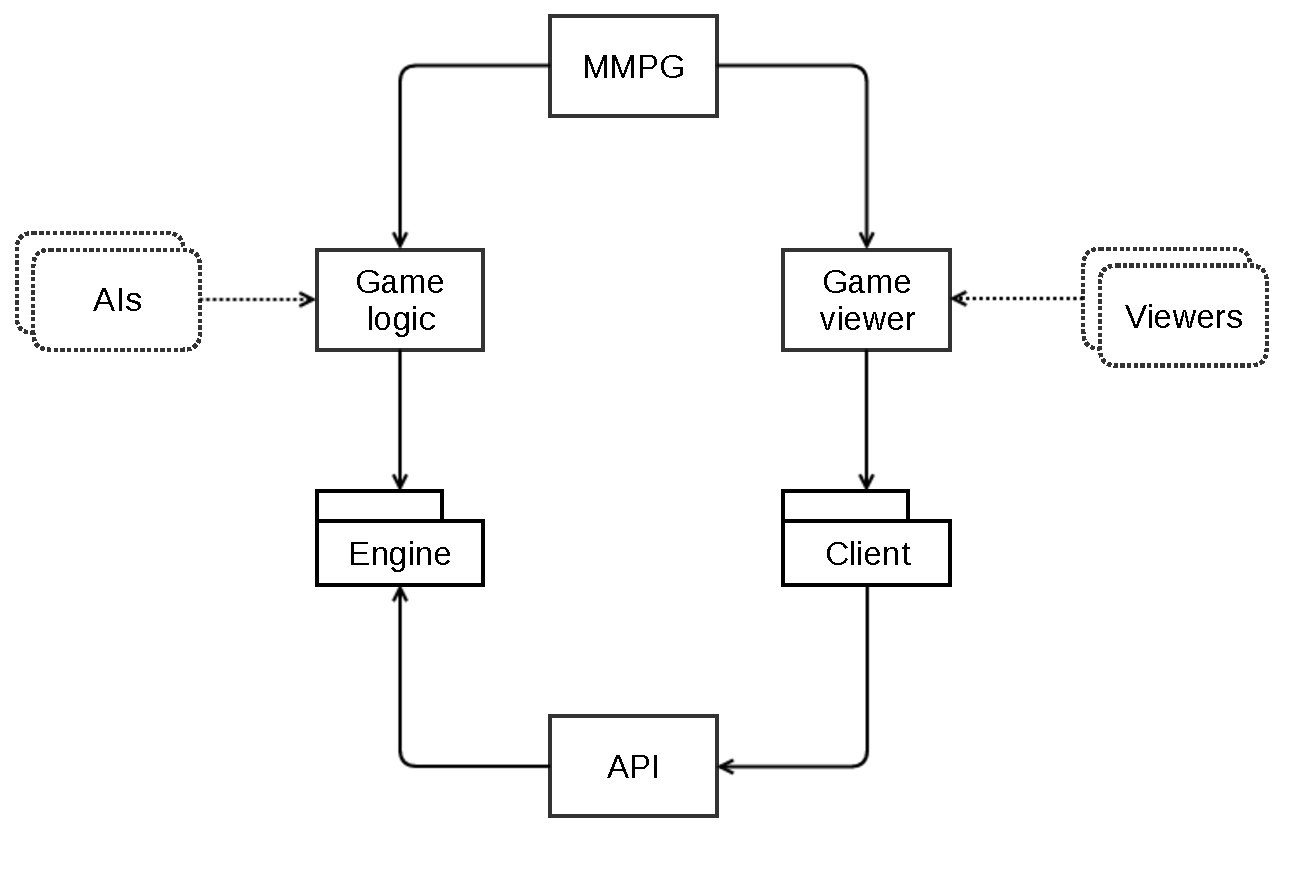
\includegraphics[scale=0.5]{graphs/mmpg_design.pdf}
\end{center}
\caption{The design of an \texttt{MMPG}}
\label{mmpg_graph}
\end{figure}
\autoref{mmpg_graph} shows a diagram of the different components that compose an \textbf{\texttt{MMPG}} and their dependencies. As it is shown,
game developers only need to implement two components to create an \textbf{\texttt{MMPG}}: the \textbf{game logic} and the \textbf{game viewer}. This is
quite logical, since these are the only two components that are game-specific.

Hence, a \textbf{massive multiplayer programming game} using the platform consists of:
\begin{description}
\item[Engine]
A library that implements basic features needed by any \texttt{MMPG}. The \textbf{engine} exposes a set
  of classes that must be extended to build the \textbf{game logic}.
\item[\texttt{API}]
A component that exposes \textbf{\texttt{HTTP}} endpoints that allow to interact with an underlying \textbf{engine}. It
  usually handles requests from a \textbf{game viewer} using the \textbf{client} library.
\item[Client]
A library that implements a set of useful classes to communicate with an \textbf{\texttt{API}} and implement
  \textbf{game viewers}.
\item[Game logic]
It includes the game world definition and the rules of the game. It is built on top of the \textbf{engine}.
\item[Game viewer]
It allows viewers to watch game matches. Also, it makes players able to upload new \textbf{\texttt{AI}}s. It uses
    the \textbf{client} library to connect to the \textbf{\texttt{API}}.
\end{description}
\clearpage
\chapter{License}
\section{Code}
The \texttt{MMPG} platform code hosted in \url{https://github.com/mmpg} will be released under
\href{https://opensource.org/licenses/MIT}{\textbf{The MIT License}}.
\section{Documents}
This monitoring report and the final document related with the \texttt{MMPG} platform and hosted in
\url{https://github.com/hecrj/mmpg} will be released under the
\href{http://creativecommons.org/licenses/by-nc-sa/4.0/legalcode.txt}{\textbf{Creative Commons Attribution-NonCommercial-ShareAlike 4.0 International}}
license.
\clearpage
\part{Planning}
\chapter{Time plan}
\section{Estimated project duration}
The project starts the \textbf{September 15th, 2015} and its deadline is the \textbf{January 25th, 2016}. Thus,
the project will take approximately \textbf{4 months} to be completed.
\section{Tasks}
This section details the different tasks and subtasks that need to be completed in order
to finish the project successfully. Every task is provided with a \textbf{description}, an \textbf{expected duration},
\textbf{possible complications} and \textbf{task dependencies}. A \textbf{time table} and a \textbf{Gantt diagram}
can be found in \autoref{planning_time_table} and \autoref{planning_timeline}, respectively.
\subsection{Project management course}
The project management course aims to help lead the project in the right direction. In this task,
different parts of the project are defined: \textbf{context and scope}, \textbf{temporal planning}, and
\textbf{economic viability}.
\begin{description}
\item[Expected duration]
75 hours.
\item[Possible complications]
None. The course is entirely guided and feedback is
  regularly provided to ensure the student can finish it properly.
\item[Task dependencies]
None.
\end{description}
\subsection{Analysis and design}
In this task, the project requirements are analyzed and a solution is designed to satisfy them.
\begin{description}
\item[Expected duration]
10 hours.
\item[Possible complications]
Some minor details might change during the implementation. It is
  important to focus on the \emph{big picture} of the project.
\item[Task dependencies]
None.
\end{description}
\subsection{Component development}
\subsubsection{Engine}
A library that will allow \textbf{game programmers} to build games and wire them to the platform
easily. The codebase will implement the features that are independent of the final game and, therefore, can be reused.
\begin{description}
\item[Expected duration]
70 hours
\item[Possible complications]
\texttt{AI} memory management might be tricky.
  The student may need to learn low-level instructions to control OS's processes.
\end{description}
\subsubsection{API}
A web-server that \textbf{notifies its subscribers of the changes that occur in the game world}.
\begin{description}
\item[Expected duration]
50 hours
\item[Possible complications]
The student needs to learn \texttt{Go}, which might take some time.
\end{description}
\subsubsection{Client}
A library that handles a connection with the \textbf{\texttt{API}}. \textbf{Game programmers} will be able to use it to build
the \textbf{real-time webviewers} of their games. It will be programmed in \texttt{}Javascript\texttt{}, using \texttt{Coffeescript}.
\begin{description}
\item[Expected duration]
30 hours
\item[Possible complications]
The student needs to learn \texttt{Coffeescript}, which might take some time.
\end{description}
\subsubsection{Control panel}
Allows \textbf{administrators} to supervise the games, start, stop and pause current matches, and obtain the
scores of every player.
\begin{description}
\item[Expected duration]
35 hours
\item[Possible complications]
The student may need some time to understand the codebase of \textbf{Jutge.org}.
\end{description}
\subsection{Game example}
A \textbf{massive multiplayer programming game} will be developed to test that the underlying
engine and infrastructure work as intended. This task will be splitted in other two: \textbf{logic} and \textbf{viewer}.
\subsubsection{Logic}
During this task, the main logic of the game will be developed on top of the \textbf{engine}.
This includes the different game \textbf{rules} and the game \textbf{world}.
\begin{description}
\item[Expected duration]
50 hours
\item[Possible complications]
Balancing the game could be \textbf{really} hard.
\item[Task dependencies]
Engine.
\end{description}
\subsubsection{Viewer}
In this task, a web-viewer that shows the game world in \textbf{real-time} will be developed using the \textbf{\texttt{API}}.
\begin{description}
\item[Expected duration]
50 hours
\item[Possible complications]
Loading a \textbf{huge} game world might be complicated.
\item[Task dependencies]
\texttt{API}.
\end{description}
\subsection{Testing and polishing}
In this task, the platform will be tested under heavy load to ensure its \textbf{stability} and \textbf{scalability}.
\begin{description}
\item[Expected duration]
40 hours
\item[Possible complications]
Components might need to change if some unexpected bottleneck is detected.
\item[Task dependencies]
Game example.
\end{description}
\subsection{Project memory}
During this task, a document explaining how the project was developed will be written.
\begin{description}
\item[Expected duration]
40 hours
\item[Possible complications]
None.
\item[Task dependencies]
Engine. It will be written in different parts, after each task is finished.
\end{description}
\subsection{Oral presentation}
Once the project memory is finished, the student will prepare the final oral presentation.
\begin{description}
\item[Expected duration]
10 hours
\item[Possible complications]
Executing live examples is risky, it might be useful to have a fallback strategy.
\item[Task dependencies]
Project memory.
\end{description}
\section{Time table}
\begin{figure}[H]
\begin{center}
\begin{tabular}{l | l}
\textbf{Task} & \textbf{Expected duration (h)}\\
\hline
Project management course & 75\\
\hline
Analysis and design & 10\\
\hline
Engine & -\\
\hspace{1em}
Learning & 5\\
\hspace{1em}
Implementation & 50\\
\hspace{1em}
Testing & 14\\
\hspace{1em}
Integration & 1\\
\hline
Client & -\\
\hspace{1em}
Learning & 10\\
\hspace{1em}
Implementation & 25\\
\hspace{1em}
Testing & 10\\
\hspace{1em}
Integration & 5\\
\hline
API & -\\
\hspace{1em}
Learning & 5\\
\hspace{1em}
Implementation & 20\\
\hspace{1em}
Testing & 3\\
\hspace{1em}
Integration & 2\\
\hline
Control panel & -\\
\hspace{1em}
Learning & 5\\
\hspace{1em}
Implementation & 20\\
\hspace{1em}
Testing & 5\\
\hspace{1em}
Integration & 5\\
\hline
Game example & -\\
\hspace{1em}
Logic & 50\\
\hspace{1em}
Viewer & 50\\
\hline
Testing and polishing & 40\\
\hline
Project memory & 40\\
\hline
Oral presentation & 10\\
\hline
\hline
\textbf{Total} & 460\\
\end{tabular}
\end{center}
\caption{Planning time table}
\label{planning_time_table}
\end{figure}
The total duration of the project is \textbf{460 hours}. The student will need to work
$\frac{460 \: hour}{16 \: week} \simeq 29 \: hour/week$ to finish the project before the deadline,
which seems reasonable.
\section{Timeline}
\begin{figure}[H]
\noindent\resizebox{\textwidth}{!}{
\begin{ganttchart}[hgrid, vgrid]{1}{25}
\gantttitle{2015}{20}
\gantttitle{2016}{5}
\\
\gantttitle{September}{5}
\gantttitle{October}{5}
\gantttitle{November}{5}
\gantttitle{December}{5}
\gantttitle{January}{5}
\\
\ganttbar{Project management}{3}{8}
\\
\ganttbar{Analysis and design}{4}{5}
\\
\ganttbar{Engine}{6}{10}
\\
\ganttbar{Client}{11}{13}
\\
\ganttbar{API}{14}{15}
\\
\ganttbar{Control panel}{16}{17}
\\
\ganttbar{Game example - logic}{11}{18}
\\
\ganttbar{Game example - viewer}{16}{20}
\\
\ganttbar{Testing and polishing}{21}{22}
\\
\ganttbar{Project memory}{11}{23}
\\
\ganttbar{Oral presentation}{24}{24}
\ganttlink{elem1}{elem2}
\ganttlink{elem2}{elem3}
\ganttlink{elem3}{elem4}
\ganttlink{elem4}{elem5}
\ganttlink{elem2}{elem6}
\ganttlink{elem4}{elem7}
\ganttlink{elem6}{elem8}
\ganttlink{elem7}{elem8}
\ganttlink{elem2}{elem9}
\ganttlink{elem9}{elem10}
\end{ganttchart}
}
\caption{Planning timeline}
\label{planning_timeline}
\end{figure}
\chapter{Budget}
\label{budget}
\section{Hardware resources}
The project will be developed using a personal desktop computer and a laptop. Also, a monitor,
a keyboard and a mouse are needed to use the desktop computer. There is no other hardware needed.
\begin{table}[H]
\centering
\begin{tabular}{l | S | S | S}
\textbf{Hardware} & \textbf{Cost (\EURtm)} & \textbf{Useful life (years)} & \textbf{Amortized cost (\EURtm)}\\
\hline
Desktop computer & 2600.00 & 4 & 34.13\\
Personal laptop & 1000.00 & 4 & 13.13\\
Monitor Acer XB270HU & 750.00 & 4 & 9.85\\
Mouse Corsair M60 & 60.00 & 4 & 0.79\\
Keyboard Corsair K70 RGB & 170.00 & 4 & 2.23\\
\hline
\hline
\multicolumn{3}{l |}{\textbf{Total}}
 & 60.13
\end{tabular}
\caption{Hardware budget}
\label{Hardware budget}
\end{table}
\section{Software resources}
All the software needed to develop the project can be used for free.
\begin{table}[H]
\centering
\begin{tabular}{l | l}
\textbf{Software} & \textbf{License}\\
\hline
Ubuntu & \url{http://www.ubuntu.com/about/about-ubuntu/our-philosophy}\\
\LaTeX{} & \url{https://latex-project.org/lppl/}\\
\texttt{git} & \url{https://git-scm.com/about/free-and-open-source}\\
\texttt{}C\texttt{++} & \url{https://gcc.gnu.org/onlinedocs/libstdc++/manual/license.html}\\
\texttt{Go} & \url{https://golang.org/project/}\\
Mozilla Firefox & \url{https://www.mozilla.org/en-US/foundation/licensing/}\\
\texttt{Coffeescript} & \url{https://github.com/jashkenas/coffeescript/blob/master/LICENSE}\\
\texttt{WebGL} & \url{https://www.khronos.org/legal/license/}\\
\end{tabular}
\caption{Software licenses}
\label{Software licenses}
\end{table}
Mozilla Firefox includes a \texttt{}Javascript\texttt{} engine and \texttt{evince} is included in Ubuntu.
Also, the \texttt{HAL} programming language is owned by the author of the project. \texttt{Jetbrains} allows students to use
\texttt{CLion} for free\footnote{\url{https://www.jetbrains.com/student/}} and
\texttt{Sublime Text} can be used without registration with no limitations\footnote{\url{http://www.sublimetext.com/2}}.
Therefore, \textbf{there are no software costs}.
\section{Human resources}
\autoref{Tasks per role} shows the tasks assigned to each project role. \autoref{Human resources budget} shows the
expected cost of the human resources according to project roles and their respective tasks.
\begin{table}[H]
\centering
\begin{tabular}{l | l | S}
\textbf{Role} & \textbf{Task} & \textbf{Time (h)}\\
\hline
\multirow{3}{*}{Project manager}
 & Project management course & 75\\
 & Project memory & 40\\
 & Oral presentation & 10\\
\hline
\multirow{1}{*}{Software engineer}
 & Analysis and design & 10\\
\hline
\multirow{6}{*}{Software developer}
 & Engine & 70\\
 & API & 50\\
 & Client & 30\\
 & Control panel & 35\\
 & Game example & 100\\
 & Testing and polishing & 40\\
\hline
\hline
\multicolumn{2}{l |}{\textbf{Total}}
 & 460.00
\end{tabular}
\caption{Tasks per role}
\label{Tasks per role}
\end{table}
\begin{table}[H]
\centering
\begin{tabular}{l | S | S | S}
\textbf{Role} & \textbf{Payment (\EURtm / h)} & \textbf{Time (h)} & \textbf{Total (\EURtm)}\\
\hline
Project manager & 35.00 & 125 & 4375.00\\
Software engineer & 40.00 & 10 & 400.00\\
Software developer & 30.00 & 325 & 9750.00\\
\hline
\hline
\multicolumn{3}{l |}{\textbf{Total}}
 & 14525.00
\end{tabular}
\caption{Human resources budget}
\label{Human resources budget}
\end{table}
\section{Other resources}
\subsection{Electricity}
Electricity will be needed to power the hardware. \autoref{Electricity budget} shows the power consumption,
the estimated time of usage, and the cost for every piece of hardware that needs an external source of power,
assuming 0.147358 \EURtm / kWh in Spain.
\begin{table}[H]
\centering
\begin{tabular}{l | S | S | S}
\textbf{Hardware} & \textbf{Consumption (W)} & \textbf{Time of usage (h)} & \textbf{Cost (\EURtm)}\\
\hline
Desktop computer & 400 & 400 & 23.58\\
Laptop & 100 & 50 & 0.74\\
Monitor Acer XB270HU & 30 & 400 & 1.77\\
\hline
\hline
\multicolumn{3}{l |}{\textbf{Total}}
 & 26.08
\end{tabular}
\caption{Electricity budget}
\label{Electricity budget}
\end{table}
\subsection{Internet connection}
An Internet connection will be necessary to perform all the tasks. The student will use its personal
internet connection most of the time, which costs 38\EURtm/month $\simeq$ 0.05\EURtm/h. It is expected to use the internet connection during the 30\% of the
total project's duration.
Thus, the estimated budget for the internet connection is
460h $\cdot$ 0.05\EURtm/h $\cdot$ 0.3 $=$ \textbf{7.28\EURtm}.
\section{Total}
\autoref{Total budget} shows the total budget needed to develop the project. The 10\% of the total cost
is added to face any unforeseen contingencies.
\begin{table}[H]
\centering
\begin{tabular}{l | S}
\textbf{Resource} & \textbf{Total cost (\EURtm)}\\
\hline
Hardware & 60.13\\
Software & 0.00\\
Human & 14525.00\\
Electricity & 26.08\\
Internet & 7.28\\
\hline
\hline
Subtotal & 14618.49\\
Contingency (10\%) & 1461.85\\
\hline
\multicolumn{1}{l |}{\textbf{Total}}
 & 16080.34
\end{tabular}
\caption{Total budget}
\label{Total budget}
\end{table}
\part{Implementation}
\chapter{Methodology}
\label{methodology}
As seen in \autoref{design}, the platform to be implemented is composed of different components that communicate with
each other. Developing a single piece of software is a difficult task, but it becomes even harder when this piece of software
communicates with other software, especially when both are being developed at the same time; changes made in
the public interface of some component can easily break other components.

Therefore, components \textbf{will} break. Developers are humans, and \textbf{humans make mistakes}. Thus, in order to be productive,
it is necessary to \textbf{detect when a component breaks as soon as possible}. That way, components can be fixed before more changes
are made and fixing it becomes a nightmare.

In order to ensure that all the components of the platform keep working during the entire implementation process, and also
detect and fix issues as soon as possible, the project was developed using an \textbf{iterative methodology} with
\textbf{continuous integration}. This methodology consisted in:
\begin{enumerate}
\item
Develop a simple prototype of the platform
\item
Run the prototype in some external server
\item
When a change is made to any component:
\begin{enumerate}
\item
Apply and integrate the change in the server
\item
Test that the prototype keeps working as expected
\end{enumerate}
\end{enumerate}
This methodology has a lot of benefits. Not only it allows to detect mistakes as soon as they are made, but it also provides
a fully working prototype of the platform that can be shown to anyone. Thus, the development progress can be shown easily and
transparently. \textbf{Stakeholders} can try the software easily while it is being developed and give \textbf{feedback}. In this case,
the prototype was available to the director of the project to assess and follow any progress closely.
\chapter{The first prototype}
The first step of the implementation process was to build a simple prototype of the platform.

This first prototype must implement the most basic feature of the platform and it also has to lay the foundations for extending
it easily. Therefore, it was decided that the first prototype should feature the first working versions of:
\begin{enumerate}
\item
The \textbf{engine}, running one simple player and notifying its actions to any subscribers.
\item
The \textbf{\texttt{API}}, subscribed to the \textbf{engine} and notifying its actions to \textbf{client}s.
\item
The \textbf{client} library, subscribed to the \textbf{\texttt{API}} and drawing the player actions in a web-browser.
\end{enumerate}
It is important to note that the \textbf{engine} and the \textbf{client} are libraries that can be used to build
game logic and game viewers, respectively. They cannot be executed as a stand-alone component. However,
game-specific code was included temporarily in this first prototype, which avoided unnecessary complexity\footnote{i.e.
creating game logic and game viewer components}.
\section{The first API}
\subsection{Programming language}
There are many programming languages that allow to create \textbf{HTTP \texttt{API}}s easily, like Pyhton, \texttt{Ruby}, \texttt{Elixir}... However,
the language chosen to implement the \textbf{\texttt{API}} was the \textbf{\texttt{Go}} programming language because it includes \textbf{native}
libraries to build concurrent \textbf{\texttt{REST} \texttt{API}}s and it is \textbf{simpler}, \textbf{faster} and \textbf{easier-to-deploy} than the alternatives.
\subsection{The subscriber hub}
The \textbf{\texttt{API}} needs to keep track of the different \textbf{client}s subscribed to it, and it also needs to be able to send data
to them.

A \textbf{subscriber hub} was developed using the native concurrency of \textbf{Go}. Basically, the \textbf{hub} runs an infinite loop in the
background that smartly monitors the connected \textbf{client}s; sending data or closing connections accordingly.
\subsection{The events endpoint}
A simple HTTP endpoint was created: \textbf{\texttt{/events}}. This endpoint accepted WebSocket connections and delegated them to the
\textbf{hub}.

After that, the \textbf{\texttt{API}} was ready to send data to \textbf{game viewers} in \textbf{real-time}.
\section{The first client}
\subsection{Programming language}
The \textbf{client} code needs to be executed by web-browsers, as \textbf{game viewers} are web-based.
Thus, it has to be written in \textbf{\texttt{Javascript}}, as it is supported by web-browsers natively.
\subsection{API subscription}
A \textbf{WebSocket} was connected to the \textbf{\texttt{/events}} endpoint, printing any received data in the \textbf{\texttt{Javascript}} console.
\section{The first engine}
\subsection{Programming language}
The \textbf{engine} needs to be \textbf{fast}, as the game logic will be built on top of it, and it also needs to access
\textbf{low-level} operative system operations, so it can limit how player programs are executed.

The most well-known programming languages that satisfiy these requirements are \texttt{C} and \texttt{C}++. However, \texttt{C}  is lacking
the capacity to \textbf{represent abstractions and interfaces} easily. Hence, \textbf{\texttt{C}++} is the perfect alternative to implement
the engine, as it is \textbf{efficient}, \textbf{object-oriented} and it has access to the \textbf{\texttt{}C\texttt{ POSIX }API\texttt{}}, which allows to talk
directly to \textbf{\texttt{UNIX}-based operative systems}.
\subsection{The first architecture}
When designing the first architecture of the \textbf{engine}, it was important to take its requirements into account:
\begin{enumerate}
\item
The \textbf{engine} must not allow \textbf{\texttt{AI}}s to cheat.
\item
\textbf{\texttt{AI}}s may be hot-swapped during a match.
\end{enumerate}
Thus, if the game logic and all the \textbf{\texttt{AI}}s were executed in the same process:
\begin{enumerate}
\item
\textbf{\texttt{AI}}s could access the memory related with the game logic or other \textbf{\texttt{AI}}s.
\item
Updating an \textbf{\texttt{AI}} would require a rebuild of the entire \textbf{game logic} and other \textbf{\texttt{AI}}s.
\item
Updating an \textbf{\texttt{AI}} would require to restart the process.
\end{enumerate}
In other words, it would be really unsafe and it would couple all the \textbf{\texttt{AI}}s and the \textbf{game logic} together.

Therefore, the initial architecture of the \textbf{engine} consisted of 2 types of processes:
\begin{description}
\item[Master process]
It represented the \textbf{game-world server}. The master process listened to requests coming from
players and notified its actions accordingly. There was only \textbf{one master process per runtime}.
\item[Player process]
It represented a \textbf{player program}. The player program contained some \textbf{\texttt{AI}} code that was
  executed \textbf{30 times per second}.
\end{description}
\autoref{engine_first_arch} shows the hierarchy of the prototype's engine runtime with $M$ players.
\begin{figure}[H]
\begin{center}
\begin{tikzpicture}[->,>=stealth',shorten >=1pt,auto,node distance=0.8cm,
    main node/.style={thick,circle,draw,minimum width=2.5cm}]

    \node[main node] (1) {master};

	\node[auto=false] (2) [below=of 1]{\ldots};

    \node[main node] (3) [left=of 2]{player$_0$};
    \node[main node] (4) [right=of 2]{player$_{M}$};


    \path (1) edge (3);
    \path (1) edge (4);
\end{tikzpicture}

\end{center}
\caption{Hierarchy of the protoype's engine processes}
\label{engine_first_arch}
\end{figure}
\subsection{Inter-process communication}
As it was explained previously, the \textbf{engine} featured a decoupled architecture. Different processes were
executed and communicated with each other using \textbf{sockets}. However, implementing inter-process communication from
scratch would have been a real challenge by itself, and it was not the subject of this project. This is where a
\textbf{messaging technology} came in.

The most well-known \textbf{messaging technologies} out there are: \texttt{RabbitMQ}, \texttt{ZeroMQ} and \texttt{ActiveMQ}.

\texttt{RabbitMQ} implements
a \textbf{broker architecture}, which means that messages are queued on a central node before being sent to its destination.
This architecture is totally unnecessary for the \textbf{engine}, as we want to decouple components, and it would also add
some \textbf{latency}.

\texttt{ActiveMQ} can be used with a \textbf{peer-to-peer architecture} but, when compared with \texttt{ZeroMQ}, it is a
\textbf{high-level} library. Thus, controlling the type of communication or socket behaviour is not easy with \texttt{ActiveMQ}.

On the other hand, \textbf{\texttt{ZeroMQ}} \cite{zeromq} is an embeddable networking library that implements
\textbf{low-latency socket communication}. It manages \textbf{low-level} communication, while providing a flexible and easy-to-use interface.
Also, \textbf{\texttt{ZeroMQ}} has bindings available for the most well-known programming languages.

Thus, \textbf{\texttt{ZeroMQ}} was the library chosen to implement all the inter-process communication.
\subsection{The first master process}
The first master process consisted of three basic components:
\begin{description}
\item[The worker]
It compiled and executed \textbf{player processes} for each given \textbf{\texttt{AI}}.
\item[The notifier]
It sent any given message through a \texttt{ZeroMQ} socket.
\item[The server]
It listened requests made by \textbf{player processes} and notified them through the \textbf{notifier}.
\end{description}
This components allowed the master process to act as a \textbf{game server}, while notifying the actions of the players to any
subscribers.
\section{Putting it all together}
Once the initial engine was finished, a simple \textbf{\texttt{AI}} was developed to simulate a player moving
while following a square shape. This way, it would be clear if the prototype worked correctly or not, as the web-viewer would need
to show this movement.

Then, the \textbf{\texttt{API}} was connected to the \textbf{engine notifier} and the received messages were directly delegated to the \textbf{\texttt{API} hub},
which in turn were sent to any open \textbf{client}s.

Finally, once the \textbf{\texttt{Javascript}} console started showing the received events, a simple scene using \textbf{\texttt{Three.js}} was created in the
\textbf{client}. This scene featured a cube representing the \textbf{player}, whose position was updated with every received event.
\autoref{cube_movement} shows the observed result. \textbf{The prototype was finished}.
\begin{figure}[H]
\begin{center}
\noindent\resizebox{!}{20em}{
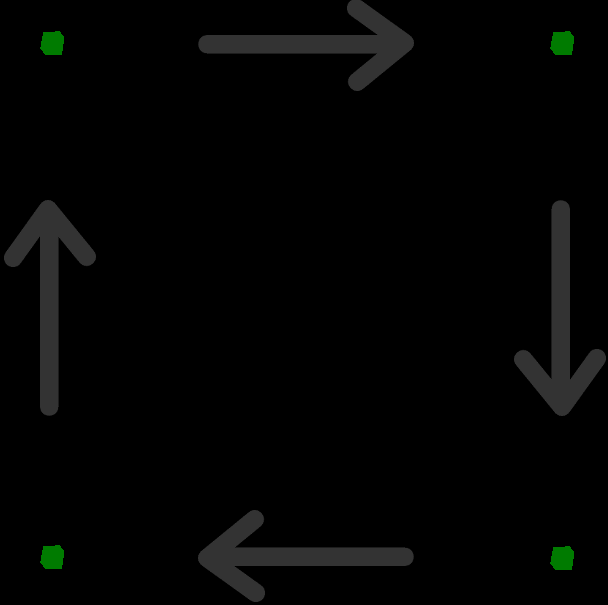
\includegraphics{images/cube_movement.png}
}
\end{center}
\caption{A cube that was moved by the player program}
\label{cube_movement}
\end{figure}
\section{Summary}
In this chapter, it is been described how the first prototype of the platform was built. A prototype that implemented the
most basic features of every component:
\begin{enumerate}
\item
The \textbf{engine} compiled and run players, and notified their actions to subscribers.
\item
The \textbf{\texttt{API}} subscribed to the engine and delegated the received events to all the connected clients.
\item
The \textbf{client} was able to connect to the \textbf{\texttt{API}} and receive events from the \textbf{engine}.
\end{enumerate}
The foundations of the platform were ready.
\chapter{Continuous integration}
Once the first prototype was finished, it was time to set up the \textbf{integration server}, as described in
\autoref{methodology}.
\section{The dedicated server}
First things first, an \textbf{integration server} to run the prototype was needed.

Initially, a server was requested to the project director. However, the university policy did not allow professors
to give root access to students. Root access was necessary because many different services might need to be installed during the
development of the platform\footnote{\texttt{ZeroMQ}, for example}. Therefore, it was decided to use an external \textbf{cloud-host provider}.

There are many providers that present cloud-hosting solutions\footnote{AWS \cite{aws}, DigitalOcean \cite{digital_ocean}, etc.}.
At the end, \textbf{Linode} \cite{linode} was the provider chosen, as the project developer already had experience with it and
the cheapest solution\footnote{This cost was covered with the contingency budget.} was enough to run the \textbf{integration server}.

A \textbf{Linode 1GB}\footnote{https://www.linode.com/pricing} running \texttt{Ubuntu} was booted up to execute an
instance of the platform.
\section{The integration service}
The next step consisted in setting up an \textbf{integration service}.

Integration services keep track of some code repositories and can be configured to \textbf{build and test the code when a change 
happens}. Additionally, most of them can be configured to \textbf{deploy changes when a build succeeds}.

As it happened with cloud-hosting providers, there are many different \textbf{integration
services}\footnote{TravisCI \cite{travis}, CircleCI \cite{circle}, etc.}. Fortunately, most of them
are \textbf{free} to use for open-source projects, like this one. At the end, \textbf{Semaphore} \cite{semaphoreci} was the chosen
\textbf{integration service}. This decision was based in the experience the project developer had with the service, as it
also happened with the cloud-hosting provider.
\section{The integration process}
\textbf{Semaphore} was configured to trigger a build when any component
changed. If a build succeeded, then \textbf{Semaphore} deployed the changes to the \textbf{Linode}, where the changes were applied.

Changes were applied in the \textbf{Linode} using \textbf{bare \texttt{git} repositories} and \textbf{script hooks}. Basically,
when some changes were pushed to the repository, a script was executed that \textbf{built and restarted the component}.
These scripts were located in the \textbf{repository itself}, so they could be updated easily with the same process.

\autoref{build_process} shows the build process of the \textbf{engine}, while \autoref{deployment_process} shows
its deployment process.
\begin{figure}[H]
\begin{center}
\noindent\resizebox{30em}{!}{
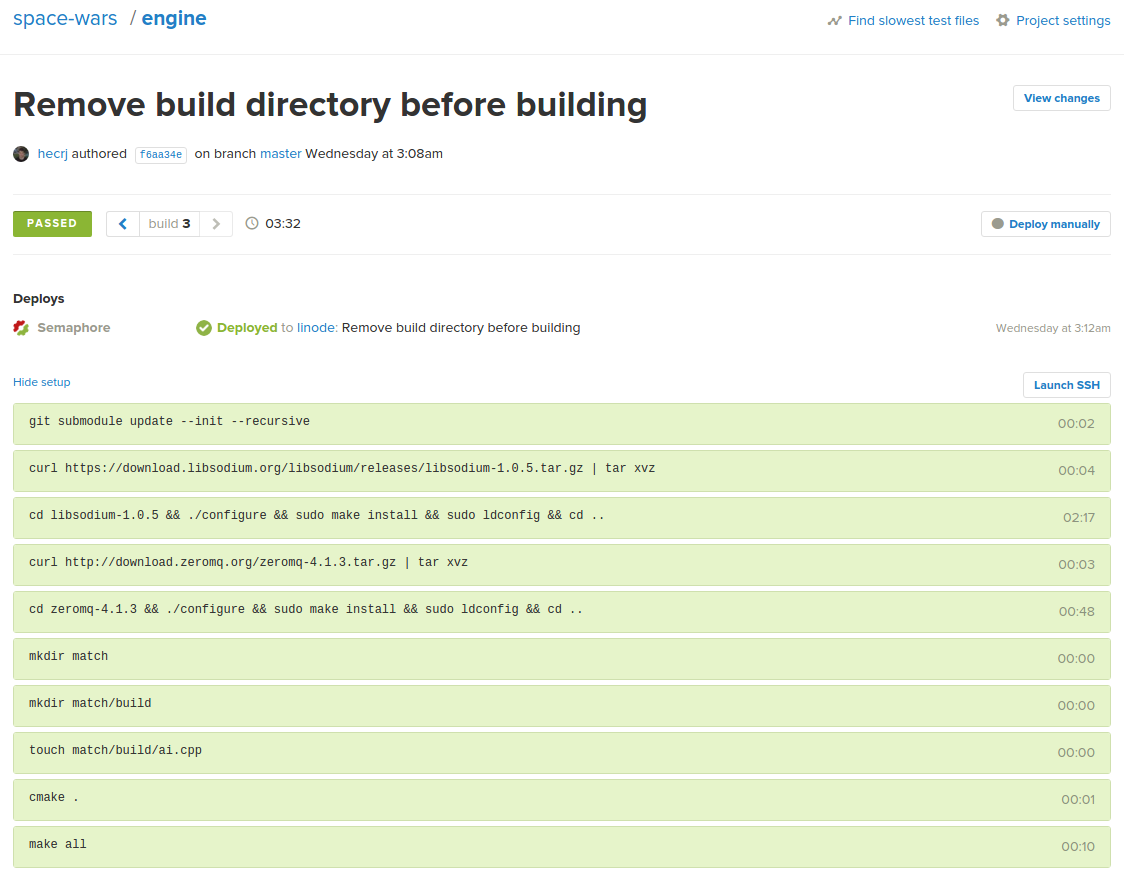
\includegraphics{images/build_process.png}
}
\end{center}
\caption{Semaphore build process}
\label{build_process}
\end{figure}
\begin{figure}[H]
\begin{center}
\noindent\resizebox{!}{30em}{
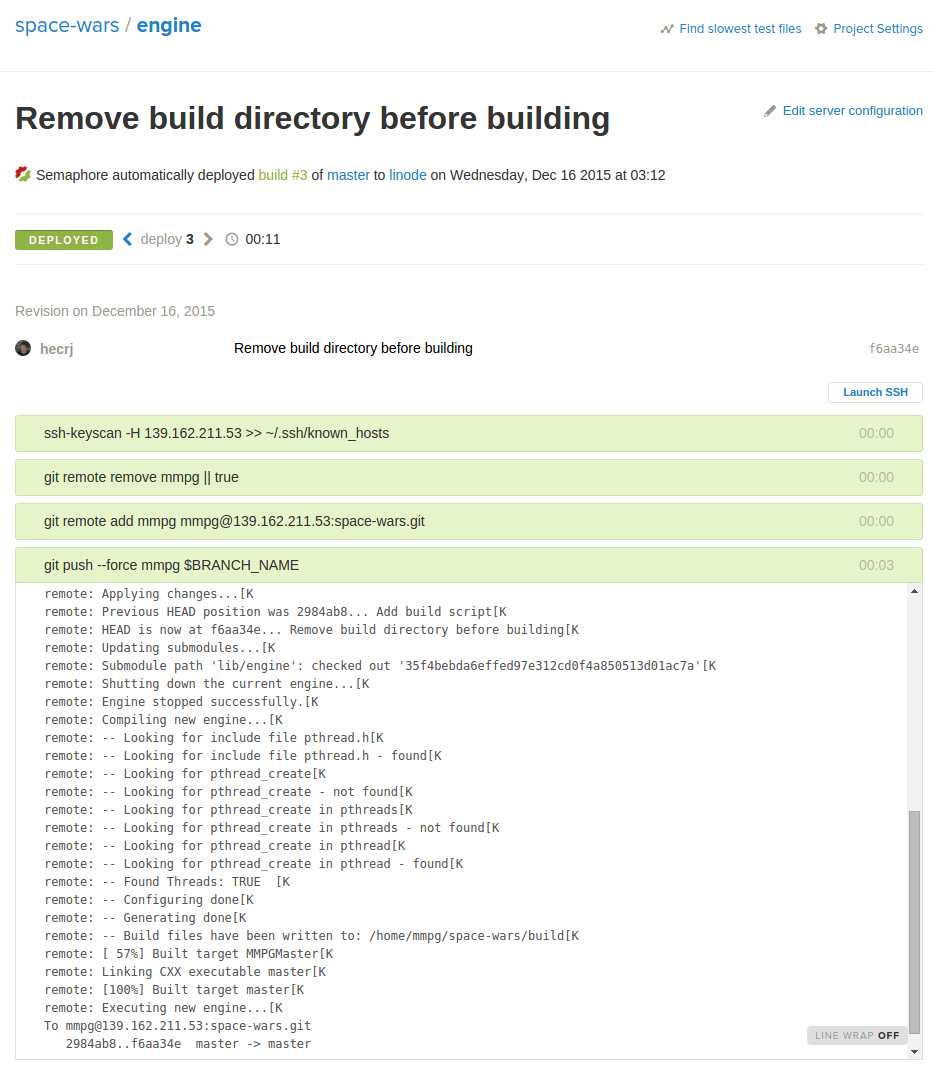
\includegraphics{images/deployment_process.png}
}
\end{center}
\caption{Semaphore deployment process}
\label{deployment_process}
\end{figure}
\chapter{The log system}
Matches of \textbf{\texttt{MMPG}}s are expected to last days or weeks, and while allowing viewers to watch the current state of
the match is mandatory, \textbf{\texttt{AI}}s will keep playing while players sleep. Therefore, \textbf{players will miss parts of the match}.
For this reason, it is important to allow viewers to replay the \textbf{past of the match}. This feature is especially
interesting, as it allows players to detect long-term strategies and learn from mistakes without the need to watch the
match constantly.

This chapter details how the replay feature was added to the platform by creating the \textbf{log system}.
\section{Event sourcing}
\textbf{Event sourcing} \cite{event_sourcing} is a technique that consists in \textbf{saving the state changes of an application as a
sequence of events}. Hence, instead of saving the current state of the application, its entire history is saved. This technique
has one main benefit: \textbf{it allows to reconstruct the state of the application at any given time}.

\textbf{Event sourcing} can be applied to the \texttt{MMPG} platform. A match can be seen as a \textbf{sequence of immutable events}:
\begin{description}
\item[Player actions]
Triggered by the different \textbf{\texttt{AI}}s.
\item[World updates]
Triggered by the \textbf{master process} to update the game world.
\end{description}
Thus, it would be possible to \textbf{recreate the match state at any given time}, if such sequence were available, by applying
all the events \textbf{from the start until that point in time}. But, as it was said before, matches can be quite long. Therefore,
processing all the events might become really time consuming.

An efficient way to solve this problem consists in saving a \textbf{snapshot} of the match periodically. That is, a big event
containing the \textbf{current state} of the match. As a consequence, it is possible to start from the \textbf{closest snapshot} in order
to recreate the state of the match at a given time.

The \textbf{event sourcing} technique with the \textbf{snapshot strategy} was used to implement replays of a match \textbf{efficiently} in
the \texttt{MMPG} platform.
\section{Logging events}
The first step to implement the replay feature was to log events in the \textbf{engine}.

The log system saved every \textbf{player action}. Additionally, a \textbf{snapshot} was also saved every second.
These \textbf{snapshots} allowed to recreate the state of the match easily and also allowed \textbf{viewers} to synchronize its state.

Internally, the log system consisted of multiple log files, where every file represented a \textbf{5-minute interval}, allowing the
retrieval of events for a particular interval of time.
\section{Delivering log files}
While \textbf{the notifier} of the \textbf{engine master process} implemented in the \textbf{first prototype} is well suited for publishing
events to subscribers, it is not able to receive data from them. For this reason, a new component was implemented in the
\textbf{master process}: the \textbf{engine app-server}.

The \textbf{app-server} was able to receive requests from another application and reply accordingly. This component creates a channel that
allows external applications to interact directly with the \textbf{engine}. The first version of this component only was able to handle
\textbf{log requests}.

A \textbf{log request} was represented by a string of characters: the \texttt{LOG} keyword followed by a space and then the UNIX time
of the log to be retrieved. For example:
\begin{verbatim}
LOG 1451606400
\end{verbatim}
This request would ask for the \textbf{log file} that contains events created at \texttt{01/01/2016 @ 00:00 (UTC)}.

Once the \textbf{engine} was able to reply to log requests, a new endpoint \textbf{\texttt{/log}} was created in the \textbf{\texttt{API}} component. This
endpoint accepted a \textbf{\texttt{time}} parameter, which was used to request the correct log file to the \textbf{engine}. Then, the log
file was sent back to the client that requested it.

Finally, the \textbf{client} library was updated to enable \textbf{log requests} in \textbf{viewers}.
\section{Compressing log files}
\textbf{Log files} had a repetitive structure, given that multiple events of the same type were stored in it. Hence, they were
really \textbf{compressible}. Moreover, \textbf{log files} were directly delivered to web-browsers through the \textbf{\texttt{API}}, and most modern
web-browsers are able to decompress \textbf{\texttt{gzip}} natively. For this reason, \textbf{log files} were compressed using \textbf{\texttt{gzip}},
\textbf{reducing both disk and bandwidth usage}.
\section{Controlling time}
Finally, a \textbf{widget} was created in the \textbf{viewer} to control the \textbf{game time}. This widget allowed to \textbf{start}, \textbf{pause},
\textbf{rewind} and \textbf{forward} the game timer. \autoref{game_time} shows the design of this widget.
\begin{figure}[H]
\begin{center}

\includegraphics{images/game_time.png}
\end{center}
\caption{Game time widget}
\label{game_time}
\end{figure}
The \textbf{game time widget} performed \textbf{log requests} under the scenes when necessary. Then, it created a \textbf{buffer} of events
from the log and started consuming them at the \textbf{same rate they were created}. When the buffer begun to empty, the \textbf{next log file
was requested to refill the buffer}.
\section{Summary}
In this chapter, the replay feature was implemented. The implementation process featured:
\begin{enumerate}
\item
Saving \textbf{player actions and snapshots} in log files.
\item
Creating an \textbf{app-server} in the \textbf{engine} to handle \textbf{log requests}.
\item
Creating a \textbf{\texttt{/log}} endpoint in the \textbf{\texttt{API}} to allow \textbf{clients} to request log files.
\item
\textbf{Compressing} log files using \textbf{\texttt{gzip}}.
\item
Developing a \textbf{game time widget} in the \textbf{viewer} to control \textbf{game time}.
\end{enumerate}
\chapter{Deployment of AI}
The next most basic feature that the platform needed to support was the \textbf{hot-swapping of \texttt{AI}}s. Players needed to be
able to change their \textbf{\texttt{AI}}s during a match.

However, it was also necessary to provide some security, so players could not change the \textbf{\texttt{AI}}s of other players. Hence,
a method to \textbf{authenticate players} was needed.

This chapter details the implementation of the authentication system and the deployment system.
\section{Recognizing players}
The first step consisted in making the \textbf{engine} acknowledge the different players by some identifier. When the \textbf{engine}
was booted up, it read a file containing a list of \textbf{user identifiers}. Then, each one of these identifiers was internally
linked with a match player.

Afterwards, a new type of request handler was added to the \textbf{app-server} developed in the previous chapter: \textbf{\texttt{PLAYER\_EXISTS}}.
This request consisted of the \texttt{PLAYER\_EXISTS} keyword followed by a space, and then a user identifier. For example:
\begin{verbatim}
PLAYER_EXISTS hector.ramon@est.fib.upc.edu
\end{verbatim}
In this example, the user identifier is an e-mail. But it is important to note that the engine was not limited to e-mails,
it was able to work with \textbf{any type of string}.

When the \textbf{engine} received a \textbf{\texttt{PLAYER\_EXISTS}} request, it checked if the given identifier was linked to some player in
the current match and replied \textbf{\texttt{YES}} or \textbf{\texttt{NO}} accordingly.
\section{Authenticating players}
The authentication system was implemented in the \textbf{\texttt{API}} component. Mainly because authentication solved an environment
limitation of the component that exposed the \textbf{engine}: the \textbf{\texttt{API}}. Hence, the \textbf{engine} did not need to know how to authenticate
users, the \textbf{\texttt{API}} did.

A new endpoint \textbf{\texttt{/auth}} was created in the \textbf{\texttt{API}}. This endpoint accepted two types of requests:
\begin{description}
\item[\texttt{POST}]
It \textbf{validated player credentials}:
\begin{enumerate}
\item
Accepted an \textbf{identifier} and a \textbf{password}.
\item
Checked whether the \textbf{identifier} and the \textbf{password} were valid using a \textbf{credentials validator}.
\item
Returned a \texttt{403 Forbidden} error if the credentials were not valid.
\item
Checked if the player existed in the \textbf{engine} using the \textbf{\texttt{PLAYER\_EXISTS}} request.
\item
Returned a \texttt{403 Forbidden} error if the player did not exist.
\item
Returned a \textbf{digitally-signed authentication token} for the given \textbf{identifier}.
\end{enumerate}
\item[\texttt{GET}]
It \textbf{renewed authentication token}s
\begin{enumerate}
\item
Accepted an \textbf{authentication token}.
\item
Checked if the \textbf{authentication token} was valid.
\item
Returned a \texttt{400 Bad Request} error if the \textbf{authentication token} was not valid.
\item
Returned a new \textbf{authentication token}.
\end{enumerate}
\end{description}
The \textbf{authentication tokens} were implemented using \textbf{\texttt{JSON WebTokens}} \cite{jwt}. This tokens have an expìration date,
hence the necessity to \textbf{renew} them.

A \textbf{credentials validator} is a simple \texttt{Go} function that tells whether the given \textbf{identifier} and
\textbf{password} are valid or not. A \textbf{credential validator} can be injected in the \textbf{\texttt{API}} easily. Hence, anyone can
implement its own \textbf{credentials validator} and customize the authentication system.

Finally, a \textbf{credentials validator} for the \textbf{Jutge.org} platform was developed using an endpoint provided by the project
director. Thus, to authenticate properly it was necessary to provide a valid \textbf{e-mail} and \textbf{password} of \textbf{Jutge.org}.
\section{Logging in players from the viewer}
Once the \textbf{authentication system} was implemented, the \textbf{client} library was updated to add support to the new \textbf{\texttt{/auth}}
endpoint. Also, a \textbf{login form} was designed in the \textbf{viewer} to allow players to \textbf{login}. \autoref{login_form}
shows how this \textbf{login form} looks.
\begin{figure}[H]
\makebox[\textwidth]{
\noindent\resizebox{!}{250pt}{

\includegraphics{images/login_ok.png}
}
\noindent\resizebox{!}{250pt}{

\includegraphics{images/login_error.png}
}
}
\caption{Login form. Valid (left). Invalid (right)}
\label{login_form}
\end{figure}
When a \textbf{login succeeded} the returned \textbf{authentication token} was saved in the \textbf{local storage} of the browser and renewed
when the \textbf{viewer} was reaccessed, or every \textbf{30 minutes} if it was kept open.
\section{Deploying new AIs}
Once, players were able to login, the deployment of new \textbf{\texttt{AI}}s could be implemented.

Firstly, a new request handler in the \textbf{app-server} was needed: \textbf{\texttt{DEPLOY\_PLAYER}}. This type of request had two
parameters: the \textbf{player identifier} and the \textbf{code of the new \texttt{AI} encoded in \texttt{base64}}. After receiving a \textbf{\texttt{DEPLOY\_PLAYER}}
request, the \textbf{engine} tried to \textbf{compile} the \textbf{code}, assigned the new executable to the player with the given \textbf{identifier},
and \textbf{restarted} its \textbf{player process}. In case the compilation failed, then the compilation error was returned.

Secondly, a new \textbf{\texttt{API}} endpoint \textbf{\texttt{/player}} was implemented to expose the new \textbf{engine} functionality and
allow \textbf{authenticated players} to change their \textbf{\texttt{AI}}s. This endpoint was pretty simple:
\begin{enumerate}
\item
Accepted an \textbf{authentication token} and an \textbf{uploaded file}.
\item
Checked whether the \textbf{authentication token} was valid or not.
\item
Returned a \textbf{\texttt{401 Unauthorized}} error if the \textbf{authentication token} was invalid.
\item
Encoded the \textbf{uploaded file} in \textbf{\texttt{base64}}.
\item
Issued a \texttt{DEPLOY\_PLAYER} request to the engine using the \textbf{identifier} in the \textbf{authentication token} and the
  \textbf{encoded file} as parameters.
\item
Returned a descriptive error if the deploymet failed.
\item
Returned a \textbf{\texttt{200 OK}} response.
\end{enumerate}
As it is been shown multiple times now. There is an \textbf{\texttt{API}} endpoint for almost every request that the \textbf{engine app-server}
can handle. Hence, the \textbf{\texttt{API}} exposes the \textbf{engine} with a layer of \textbf{control} on top of it.

Finally, the \textbf{client} was updated to support the new endpoint and a \textbf{deployment form} was created in the \textbf{viewer}.
This form was designed having in mind that \textbf{the deployment process should be fun}, so players feel encouraged to
\textbf{improve its code}. \autoref{deploy_error} shows how the \textbf{deployment form} looks.
\begin{figure}[H]
\makebox[\textwidth]{
\noindent\resizebox{!}{210pt}{
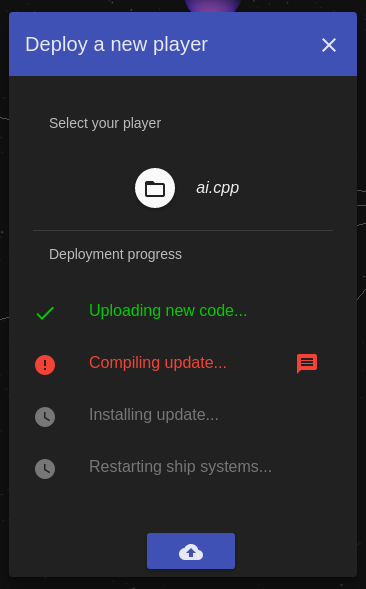
\includegraphics{images/deploy_error.png}
}
}
\caption{Player deployment with a compilation error}
\label{deploy_error}
\end{figure}
\section{Summary}
Summarizing, this capter detailed the implementation of:
\begin{enumerate}
\item
An \textbf{authentication system}, which consisted in:
\begin{enumerate}
\item
Implementing the \textbf{\texttt{PLAYER\_EXISTS}} handler in the \textbf{engine app-server}.
\item
Adding of the \textbf{\texttt{/auth}} endpoint to the \textbf{\texttt{API}}.
\item
Creating of the \textbf{login form} in the viewer.
\end{enumerate}
\item
The \textbf{\texttt{AI} hot-swapping} feature, which consisted in:
\begin{enumerate}
\item
Implementing the \textbf{\texttt{DEPLOY\_PLAYER}} handler in the \textbf{engine app-server}.
\item
Adding of the \textbf{\texttt{/player}} endpoint to the \textbf{\texttt{API}}.
\item
Creating of the \textbf{deployment form} in the viewer.
\end{enumerate}
\end{enumerate}
\chapter{The first game world}
[...]
\section{Choosing a game: Space Wars}
[...]
\section{Generating a planetary system procedurally}
[...]
\section{Rendering the planetary system}
[...]
\section{Summary}
[...]
\chapter{Fleets and planets}
[...]
\section{Generating ships in conquered planets}
[...]
\section{Moving fleets between planets}
[...]
\section{Summary}
[...]
\chapter{A whole galaxy}
[...]
\section{Generating multiple planetary systems}
[...]
\section{Separating world structure from dynamic data}
[...]
\section{Rendering a galaxy}
[...]
\section{Connecting planetary systems}
[...]
\section{Summary}
[...]
\part{Evaluation}
\chapter{Validation}
\label{validation}
\section{Continuous integration}
[...]
\section{Testing}
[...]
\chapter{Time management}
\section{Time table}
\begin{figure}[H]
\begin{center}
\noindent\resizebox{!}{16em}{
\begin{tabular}{l | l}
\textbf{Task} & \textbf{Expected duration (h)}\\
\hline
Project management course & 75\\
\hline
Analysis and design & 10\\
\hline
Game engine & -\\
\hspace{1em}
Learning & 5\\
\hspace{1em}
Implementation & 50\\
\hspace{1em}
Testing & 14\\
\hspace{1em}
Integration & 1\\
\hline
Real-time notifier & -\\
\hspace{1em}
Learning & 10\\
\hspace{1em}
Implementation & 25\\
\hspace{1em}
Testing & 10\\
\hspace{1em}
Integration & 5\\
\hline
Notifier subscriber & -\\
\hspace{1em}
Learning & 5\\
\hspace{1em}
Implementation & 20\\
\hspace{1em}
Testing & 3\\
\hspace{1em}
Integration & 2\\
\hline
Control panel & -\\
\hspace{1em}
Learning & 5\\
\hspace{1em}
Implementation & 20\\
\hspace{1em}
Testing & 5\\
\hspace{1em}
Integration & 5\\
\hline
Game example & -\\
\hspace{1em}
Logic & 50\\
\hspace{1em}
Real-time viewer & 50\\
\hline
Testing and polishing & 40\\
\hline
Project memory & 40\\
\hline
Oral presentation & 10\\
\hline
\hline
\textbf{Total} & 460\\
\end{tabular}
}
\end{center}
\caption{Time table}
\label{time_table}
\end{figure}
[...]
\section{Timeline}
\begin{figure}[H]
\makebox[\textwidth]{
\noindent\resizebox{300pt}{!}{
\begin{ganttchart}[hgrid, vgrid]{1}{25}
\gantttitle{2015}{20}
\gantttitle{2016}{5}
\\
\gantttitle{September}{5}
\gantttitle{October}{5}
\gantttitle{November}{5}
\gantttitle{December}{5}
\gantttitle{January}{5}
\\
\ganttbar{Project management}{3}{11}
\\
\ganttbar{Analysis and design}{6}{7}
\\
\ganttbar{Engine}{9}{15}
\\
\ganttbar{API}{9}{13}
\\
\ganttbar{Client}{9}{13}
\\
\ganttbar{Space Wars - logic}{16}{19}
\\
\ganttbar{Space Wars - viewer}{16}{20}
\\
\ganttbar{Testing and polishing}{21}{22}
\\
\ganttbar{Project memory}{16}{23}
\\
\ganttbar{Oral presentation}{24}{24}
\ganttlink{elem1}{elem2}
\ganttlink{elem1}{elem3}
\ganttlink{elem1}{elem4}
\ganttlink{elem2}{elem5}
\ganttlink{elem3}{elem6}
\ganttlink{elem4}{elem6}
\ganttlink{elem5}{elem7}
\ganttlink{elem6}{elem7}
\ganttlink{elem8}{elem9}
\end{ganttchart}
}
}
\caption{Final timeline}
\label{gantt_current}
\end{figure}
\section{Dedication}
\autoref{dedication} shows the \textbf{relative amount of contributions per day} to this project.
\begin{figure}[H]
\makebox[\textwidth]{
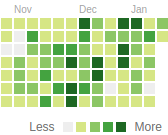
\includegraphics[scale=0.6]{images/dedication.png}
}
\caption{GitHub contributions to the \texttt{MMPG} project \url{https://github.com/hecrj}}
\label{dedication}
\end{figure}
As it can be observed, there is \textbf{at least one contribution per day since November 4}. However, while dedication has
been constant, there are many days where \textbf{contributions were minimal}. Hence, \textbf{dedication and productivity are expected
to increase} during the incoming holidays.
\chapter{Economic cost}
\section{Hardware resources}
The project used the hardware resources specified in \fullref{budget}. However, a \textbf{Linode 1GB} was needed during \textbf{3 months}.
\begin{table}[H]
\centering
\begin{tabular}{l | S}
\textbf{Hardware} & \textbf{Cost (\EURtm)}\\
\hline
Hardware budget & 60.13\\
Linode 1GB & 27.47\\
\multicolumn{1}{l |}{\textbf{Total}}
 & 87.60
\end{tabular}
\caption{Hardware cost}
\label{Hardware cost}
\end{table}
\section{Software resources}
As stated in the original planning, all the software needed to develop the project can be used for free.
  \autoref{additional_software} shows additional software that was used but it was not listed in the original planning.
\begin{table}[H]
\centering
\begin{tabular}{l | l}
\textbf{Software} & \textbf{License}\\
\hline
\texttt{Three.js} & \url{https://github.com/mrdoob/three.js/blob/master/LICENSE}\\
\end{tabular}
\caption{Additional software}
\label{Additional software}
\end{table}
\section{Human resources}
\autoref{Human resources cost} shows the final cost of the human resources according
to the final task durations detailed in \autoref{time_table} and the task per role in \autoref{Tasks per role}.
\begin{table}[H]
\centering
\begin{tabular}{l | S | S | S}
\textbf{Role} & \textbf{Payment (\EURtm / h)} & \textbf{Time (h)} & \textbf{Total (\EURtm)}\\
\hline
Project manager & 35.00 & 125 & 4375.00\\
Software engineer & 40.00 & 10 & 400.00\\
Software developer & 30.00 & 325 & 9750.00\\
\hline
\hline
\multicolumn{3}{l |}{\textbf{Total}}
 & 14525.00
\end{tabular}
\caption{Human resources cost}
\label{Human resources cost}
\end{table}
\section{Other resources}
\subsection{Electricity}
\autoref{Electricity cost} shows the electricity cost of the project.
\begin{table}[H]
\centering
\begin{tabular}{l | S | S | S}
\textbf{Hardware} & \textbf{Consumption (W)} & \textbf{Time of usage (h)} & \textbf{Cost (\EURtm)}\\
\hline
Desktop computer & 400 & 400 & 23.58\\
Laptop & 100 & 50 & 0.74\\
Monitor Acer XB270HU & 30 & 400 & 1.77\\
\hline
\hline
\multicolumn{3}{l |}{\textbf{Total}}
 & 26.08
\end{tabular}
\caption{Electricity cost}
\label{Electricity cost}
\end{table}
\subsection{Internet connection}
The project was developed using the internet connection described in \fullref{budget}. The internet connection was used
approximately during the 30\% of the total project's duration, as expected.
Thus, the final cost of the internet connection was 460h $\cdot$ 0.05\EURtm/h $\cdot$ 0.3 $=$ \textbf{7.28\EURtm}.
\section{Total}
\autoref{Total cost} shows the total cost of the project.
\begin{table}[H]
\centering
\begin{tabular}{l | S}
\textbf{Resource} & \textbf{Total cost (\EURtm)}\\
\hline
Hardware & 87.60\\
Software & 0.00\\
Human & 14525.00\\
Electricity & 26.08\\
Internet & 7.28\\
\hline
\hline
\multicolumn{1}{l |}{\textbf{Total}}
 & 14645.96
\end{tabular}
\caption{Total cost}
\label{Total cost}
\end{table}
\chapter{Sustainability}
This section contains a sustainability report of the project based on the application of the matrix described by
Christian Felber in `The economy of the common good' \cite{sustainability_report}. However, only the \textbf{planning}
stage is considered.
\section{Economic analysis}
The economical analysis is complete and thorough, all costs are assessed and reasonable.
Resources are used efficiently, spending more time in the most important tasks. Moreover, the best technologies
are chosen to produce the best results in the least amount of time possible. A contingency budget has been added
to take care of any unexpected problems. However, the project is not aimed to be profitable, so there will be
no direct economic benefit from it.
\\[0.1cm]
Overall, the project receives a 7 in economical viability because its efficency but lack of profitability.
\section{Social impact analysis}
The project is directed to computer science students and teachers, and game progammers. The project
will be used by students to learn different programming techniques, by teachers to evaluate these students, and
by game programmers to create new content. Moreover, it will be used in the Data Structures and Algorithms subject
at the Barcelona School of Informatics (\textbf{FIB}). The project will make the learning process more fun, it will also
reduce the amount of work for teachers, and it will make game programmers able to create entertaining games easily.
However, the project will not affect the mainstream consumer directly. It will only be relevant inside a specific
community in computer science.
\\[0.1cm]
The project receives a 6 in social impact because it will be positive for a specific community but it will not
have a direct impact on the global population.
\section{Environmental impact analysis}
The project will use 177kWh of electricity, which is approximately 174kg
of CO\textsuperscript{2} \cite{co2}. This is the amount of CO\textsuperscript{2} that a car produces by driving only 7
hours\footnote{\url{http://www.yousustain.com/footprint/howmuchco2?co2=174+kg}}. Also, any source of
information will be accessed digitally over the internet. However, the hardware can not be fully
recycled and it will, eventually, become electronic waste with a high amount of contaminants.
\\[0.1cm]
The project obtains an 8 in environmental impact because its environmental footprint is almost negligible.
\section{Matrix}
\autoref{Sustainability matrix} shows the sustainability matrix and the total score obtained in the planning
stage. The total score obtained is \textbf{21 out of 30}. Therefore, the project is planned to be \textbf{reasonably sustainable}.
\begin{table}[H]
\centering
\begin{tabular}{c | c | c | c | c}
\textbf{Sustainable?} & \textbf{Economic} & \textbf{Social} & \textbf{Environmental} & \textbf{Total}\\
\hline
Planning & 7 & 6 & 8 & \textbf{21}\\
\end{tabular}
\caption{Sustainability matrix}
\label{Sustainability matrix}
\end{table}
\chapter{Legality}
There are no special laws that apply to this project. The entity using the platform
is liable for the information inputted in it, as it is specified in the \textbf{code license}.
\chapter{Conclusion}
...
\bibliographystyle{plain}
\bibliography{references}
\end{document}
